\documentclass[10pt,a4paper]{article}
\usepackage[margin=2cm]{geometry}
\usepackage[T1]{fontenc}
\usepackage{lmodern}
\usepackage{amsmath,amssymb}
\usepackage{booktabs,longtable,array,multirow}
\usepackage{graphicx}
\usepackage{xcolor}
\usepackage{verbatim}
\usepackage{float}
\usepackage{enumitem}
\usepackage[hidelinks]{hyperref}
\setlist{nosep,leftmargin=*}
\newcommand{\pos}[1]{\textbf{#1}}
\newcommand{\ci}[2]{\,{\scriptsize[#1,\,#2]}}
\setlength{\tabcolsep}{4pt}

\title{Cross-Task Transfer with Dr.~GRPO on Qwen3.5-2B:\\
SOLVE, JUDGE, RECONSTRUCT and a Mixed-Task Model\\[4pt]
\large Full end-to-end report: setup, methods, run settings, results}
\author{ANLP project (Turing cluster runs, 2026-10-06 to 2026-10-08)}
\date{8 October 2026}

\begin{document}
\maketitle

\begin{abstract}
We train the post-trained \texttt{Qwen/Qwen3.5-2B} with Dr.~GRPO (LoRA) on three mathematical tasks built from
DeepMath-103K: SOLVE (solve a problem), JUDGE (find the first wrong step of a worked solution) and RECONSTRUCT (recover
a question from its answer and clues). We train one model per task and one model on an equal mixture of the three
tasks, then evaluate every model on all three 400-question test sets.

Each single-task model gains strongly on its own task: SOLVE $+16.6$ accuracy points, JUDGE $+17.2$ error-finding
points, RECONSTRUCT $+21.4$ rubric points. Transfer across tasks is mixed: RECONSTRUCT training costs $-10.7$ on
SOLVE.

The mixed-task model (balanced 10/10/10 batches, lr $2\times10^{-5}$) improves every task with no negative transfer:
SOLVE $+17.1$, JUDGE error-finding $+32.2$ (Youden's $J$ $+45.4$), RECONSTRUCT $+18.3$. It matches the SOLVE
specialist, beats the JUDGE specialist, and comes within 3 points of the RECONSTRUCT specialist.

The report also documents why the first SOLVE recipe failed ($-2.2$) and how it was fixed: a larger batch, a lower
learning rate and a stricter, audited answer checker. All numbers use 95\% paired bootstrap intervals.
\end{abstract}

\tableofcontents
\newpage

%=====================================================================================================================
\section{Headline results}

\begin{table}[H]
\centering\small
\caption{Transfer matrix on the test sets: $\Delta$ against the untrained Qwen3.5-2B (points, paired, 95\% bootstrap
CI). Bold marks the model's own training task. JUDGE step\,\% is error-finding (an incorrect solution judged
incorrect \emph{and} the exact first wrong step named); Youden's $J$ is verdict accuracy on incorrect plus on correct
solutions minus 100.}
\label{tab:headline}
\resizebox{\linewidth}{!}{%
\begin{tabular}{lrrrr}
\toprule
Trained on $\downarrow$ / measured on $\rightarrow$ & SOLVE accuracy & JUDGE step\,\% & JUDGE Youden $J$ & RECONSTRUCT PC-v4\\
\midrule
SOLVE only (step 66)       & \pos{+16.6}\ci{+13.8}{+19.1} & +8.8\ci{+2.1}{+16.1} & +15.4\ci{+6.2}{+23.8} & +3.8\ci{+1.4}{+6.3}\\
JUDGE only (step 26)       & $-1.1$\ci{$-4.1$}{+1.9} & \pos{+17.2}\ci{+10.2}{+24.0} & \pos{+28.4}\ci{+19.5}{+36.9} & +6.0\ci{+3.3}{+8.6}\\
RECONSTRUCT only (step 104)& $-10.7$\ci{$-13.7$}{$-7.7$} & +14.2\ci{+7.2}{+21.8} & +7.9\ci{$-1.2$}{+17.0} & \pos{+21.4}\ci{+19.1}{+23.5}\\
\midrule
Mixed, 1/3 each (step 75)  & \pos{+17.1}\ci{+14.3}{+19.9} & \pos{+32.2}\ci{+25.9}{+38.6} & \pos{+45.4}\ci{+37.4}{+52.6} & \pos{+18.3}\ci{+16.1}{+20.5}\\
\bottomrule
\end{tabular}}
\end{table}

\begin{figure}[H]
\centering
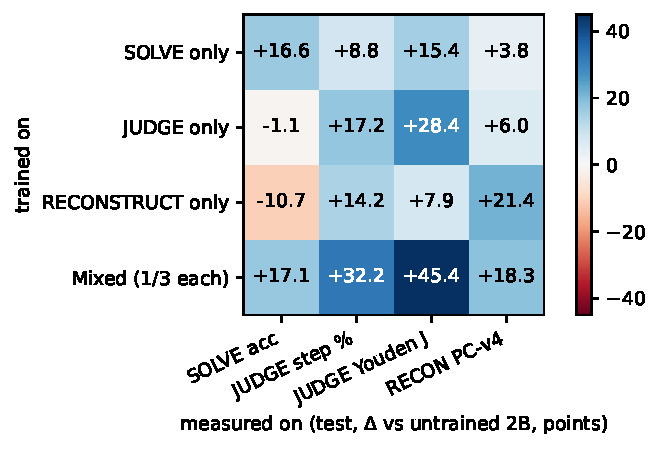
\includegraphics[width=0.62\linewidth]{figures/transfer_heatmap.pdf}
\caption{The transfer matrix of Table~\ref{tab:headline} as a heatmap.}
\end{figure}

\paragraph{Main findings.}
\begin{enumerate}
\item \textbf{The mixed-task model is the best overall:}
  \begin{itemize}
  \item on SOLVE, equal to the SOLVE specialist ($+0.6$, not significant);
  \item on JUDGE, far better than the JUDGE specialist (error-finding $+15.0$, $J$ $+17.0$);
  \item on RECONSTRUCT, 3 points below the RECONSTRUCT specialist ($-3.0$) but better on same-question recovery
        ($+8.0$) and on mathematical validity;
  \item every cross-task cell is positive.
  \end{itemize}
\item \textbf{Every single-task model improves strongly on its own task.}
\item \textbf{Single-task transfer is uneven:}
  \begin{itemize}
  \item SOLVE helps both other tasks;
  \item JUDGE helps RECONSTRUCT and leaves SOLVE unchanged;
  \item RECONSTRUCT hurts SOLVE ($-10.7$), and its JUDGE error-finding gain comes with more false alarms ($+10.2$).
  \end{itemize}
\item \textbf{SOLVE needed a new recipe.} With lr $5\times10^{-5}$ and 8 questions per step it gave $-2.2$; with lr
  $10^{-5}$ and 32 questions per step it gave $+16.6$ (Section~\ref{sec:solve}).
\end{enumerate}

%=====================================================================================================================
\section{Tasks, data and prompts}

\subsection{Model}
\begin{itemize}
\item \textbf{Student:} \texttt{Qwen/Qwen3.5-2B}, post-trained, non-thinking chat template. Every run starts from it.
\item \textbf{Reference:} \texttt{Qwen/Qwen3.5-9B}, evaluated identically and never trained.
\item \textbf{Final test judge:} \texttt{Qwen/Qwen3.8-27B}, used only for judging (Section~\ref{sec:scoring}).
\end{itemize}

\subsection{Data (FINAL-v3)}
\begin{itemize}
\item \textbf{Source:} all questions come from DeepMath-103K (difficulty 5--9).
\item \textbf{Split per task:} 4,000 rows each, 3,600 train and 400 test.
\item \textbf{Disjoint and matched:} the three tasks use different questions, matched on topic and difficulty.
\item \textbf{Dev slice:} a seeded 200-question slice of each train split is never trained on; it is used for
      checkpoint checks. That leaves 3,400 training questions per task.
\item \textbf{Training order:} every run uses the same seeded shuffle of those 3,400 (the ``matrix order'').
\item \textbf{Leakage check:} no dev or test question appears in any run's training prompts.
\end{itemize}

\begin{table}[H]
\centering\small
\caption{The three tasks.}
\begin{tabular}{p{2.2cm}p{4.2cm}p{4.6cm}p{4.6cm}}
\toprule
Task & Input & Output & How correctness is decided\\
\midrule
SOLVE & a maths problem & a worked solution with one \texttt{<final\_answer>} tag & the answer equals the key (checker v3, deterministic)\\
JUDGE & a problem and a worked solution split into steps S1\dots Sn (correct, or with one first error) & \texttt{Decision: correct/incorrect}, \texttt{First wrong step: Sk/none}, an explanation & verdict and step against the key (parser); explanation by an LLM judge\\
RECONSTRUCT & a final answer and clues (observations) about a hidden question & one JSON object with \texttt{question}, \texttt{assumptions}, \texttt{justification} & fidelity to the hidden question and validity, by an LLM judge\\
\bottomrule
\end{tabular}
\end{table}

\subsection{Prompts and strict gates}
\textbf{Prompts.} The student prompts are version v2 (\texttt{baseline.PROMPT\_FILES}). Each asks for one final
block, carries a brevity line, and states the gate rules.

\textbf{Strict gates} (\texttt{strict\_gates.py}) run before any score or reward; a failed gate scores 0.
\begin{itemize}
\item \textbf{SOLVE:} several \texttt{<final\_answer>} tags that disagree.
\item \textbf{JUDGE:} several or contradictory decisions or steps, or a decision/step mismatch.
\item \textbf{RECONSTRUCT:} the answer written into the question, monologue or drafting, or no question. The answer
      is parsed from the last JSON object.
\end{itemize}

%=====================================================================================================================
\section{Scoring and evaluation protocol}
\label{sec:scoring}

\subsection{SOLVE answer checker (v3)}
\texttt{solution\_verification.compare\_answer\_detailed} is used for the training reward, every evaluation and the
gates. It is deterministic and uses no LLM. Its layers run in order; layers 2--5 can only turn a non-correct
decision into ``correct'':
\begin{enumerate}
\item \textbf{Rules:}
  \begin{itemize}
  \item normalised exact match, booleans (with \emph{true/false} = \emph{yes/no}), letter choices;
  \item exact rational arithmetic, congruences, intervals;
  \item SymPy equivalence;
  \item notation fixes: $\geq$ variants, \verb|\bmod|, \verb|\ln 2|, $+\infty$, degrees, \verb|\sqrt[n]{}|, $|x|$.
  \end{itemize}
\item \textbf{Cleaned answer forms:}
  \begin{itemize}
  \item a variable assignment such as $n=2^k$ or $(p,q)=(2,2)$, or $x=0,y=0,z=0$ read as a tuple;
  \item a trailing qualifier such as ``for $k\ge1$'' removed.
  \end{itemize}
  A cleaned form must be pure mathematics, and a removed part may not contain hedge words (\emph{or, not, maybe,
  approximately}, \dots).
\item \textbf{Equation chains:} the last side counts as the answer.
\item \textbf{Numeric closeness:}
  \begin{itemize}
  \item exact numbers must be equal exactly;
  \item a decimal key with $\ge4$ decimals fixes the precision;
  \item infinities are never compared numerically.
  \end{itemize}
\item \textbf{DeepMath's official checker pair:} OpenMathInstruct's \texttt{math\_equal} (vendored; tolerance
      tightened from $10^{-4}$ to $10^{-9}$; Python \texttt{eval} paths removed), then \texttt{math-verify}. Both
      only see pure-mathematics answers that list no more values than the key.
\item \textbf{Time limit:} 10\,s per check. The main thread uses an alarm; checks from trainer threads run in a process
      pool.
\end{enumerate}

\textbf{Audit} on 7,465 distinct (key, answer) pairs from training rollouts and test outputs:
\begin{itemize}
\item 161 unverified and 8 wrong decisions became correct. Each was inspected by hand.
\item 1 correct decision was lost (a hedged answer).
\item The false positives found during development are now regression tests:
  \begin{itemize}
  \item 88327 accepted for 88329 (DeepMath's $10^{-4}$ tolerance);
  \item \texttt{True} accepted for 1;
  \item $a\neq3$ read as 3;
  \item ``3 or 5'' accepted for 3;
  \item prose such as ``does not converge to 0'' accepted for 0;
  \item $2^{2^{\aleph_0}}$ accepted for $2^{\aleph_0}$ (\texttt{math-verify}).
  \end{itemize}
\end{itemize}
The untrained model moves from 50.2 to 52.4 (dev) and from 51.0 to 52.6 (test). \textbf{Every SOLVE number in this
report uses v3}; older evaluations were re-scored.

\subsection{Judges}
\begin{itemize}
\item \textbf{Final test scores for JUDGE (V/L/E/M) and RECONSTRUCT (PC-v4, same question):} \texttt{Qwen3.8-27B} as a
      logit-reading judge (\texttt{qwen\_judging.py}): one generated token at temperature 0, probability-weighted
      levels, calibrated cutoffs. Its agreement with DeepSeek on total scores is $r=0.940$ (JUDGE) and $0.840$
      (RECONSTRUCT).
\item \textbf{Training rewards and RECONSTRUCT dev scoring:} the Jev API (\texttt{jev-1.13.0},
      \texttt{jev\_judging.py}): gate $\rightarrow$ few-shot shortcut stage $\rightarrow$ calibrated questions.
\end{itemize}
The judge that selects or rewards a model is never the one that gives its final test score.

\subsection{Evaluation protocol}
\begin{itemize}
\item \textbf{Sampling:} temperature 1.0, top-$p$ 1.0, seed 0; a 16k-token first pass, continued to 32k for answers
      that hit 16k.
\item \textbf{Samples per question:} SOLVE 4. JUDGE and RECONSTRUCT 1 for trained models; 4 for the untrained 2B and
      the 9B, whose mean over samples estimates the same single-sample score.
\item \textbf{Statistics:} deltas are paired on the same questions; 95\% bootstrap over questions, 2,000 resamples.
\end{itemize}

\subsection{Metrics}
\begin{itemize}
\item \textbf{SOLVE accuracy:} a strict (gated) verified answer; pass@1 is the mean over 4 samples. \textbf{pass@4:}
      at least one of 4 correct.
\item \textbf{JUDGE step\,\% (error-finding)}, on the 200 solutions that contain an error: the verdict is
      ``incorrect'' \emph{and} the exact first wrong step is named.
\item \textbf{JUDGE false alarm\,\%:} a correct solution judged incorrect (lower is better).
\item \textbf{JUDGE Youden's $J$:} verdict accuracy on incorrect solutions $+$ on correct solutions $-100$. A
      one-verdict model scores 0. On this balanced 200/200 set, $J = 2\times$verdict accuracy $-100$.
\item \textbf{JUDGE V/L/E/M (/100):} the 27B rubric for verdict, location, explanation and mathematical soundness.
\item \textbf{RECONSTRUCT PC-v4 (/100):} the 27B rubric for premise fidelity (P), target fidelity (T), evidence use (E)
      and mathematical validity (M). Shortcuts and gated answers score 0.
\item \textbf{RECONSTRUCT same question\,\%:} judged equivalent to the hidden original.
\end{itemize}
Combined JUDGE accuracy (verdict and step, with ``none'' counted as the step on correct solutions) rewards a bias
toward answering ``correct''. It is reported only next to the per-label split.

%=====================================================================================================================
\section{Training method: Dr.~GRPO}

\subsection{Objective}
For each question, $G=8$ answers $o_1,\dots,o_G$ are sampled and each gets a reward $r_i\in[0,1]$.
\begin{align}
\hat A_i &= r_i - \tfrac1G\textstyle\sum_{j} r_j \qquad\text{(no division by the standard deviation)}\\
\mathcal L &= -\frac{1}{N_{\text{kept}}}\sum_{i}\sum_{t}\frac{\rho_{it}\,\hat A_i\,\log\pi_\theta(o_{it}\mid q,o_{i,<t})}{16384},
\qquad \rho_{it}=\min\!\Bigl(2,\;e^{\log\pi_\theta-\log\pi_{\text{vLLM}}}\Bigr)
\end{align}
\begin{itemize}
\item \textbf{Normalizer:} the constant 16,384 (the generation cap), not each answer's length (Dr.~GRPO).
\item \textbf{Updates:} one optimizer update per batch, so there is no PPO clipping. KL coefficient $\beta=0$.
\item \textbf{Dropped questions:} those whose answers all got the same reward, since they have no signal.
\item \textbf{Truncated answers} stay in their group with reward 0.
\item \textbf{Overlapped rollouts} (\texttt{async\_rollouts}): the answers for step $s{+}1$ are generated with the
      adapter of step $s$ while step $s$ trains. That is a one-update lag, corrected by $\rho$; it cut SOLVE's step
      time from 15 to $\approx$8 minutes.
\end{itemize}

\subsection{Rewards (\texttt{rewards.py})}
\begin{itemize}
\item \textbf{SOLVE:} $r=1$ if the single final answer is verified correct (checker v3), else 0.
\item \textbf{JUDGE:} $r=0$ for a wrong verdict; otherwise $r = 0.5 + 0.25\cdot[\text{first wrong step right}] +
      0.25\cdot\min(8,E+M)/8$. Here $E$ (explanation) and $M$ (soundness) are 0--4 Jev levels, probability-weighted.
\item \textbf{RECONSTRUCT:} $r = 6.25\,(P+T+E+M)/100 - 0.1\cdot[\text{several drafts}]$, floored at 0, with P, T, E,
      M from Jev (0--4 each). A shortcut (answer copied, copy-only, no usable question) or a gated answer scores 0.
\item \textbf{Every task:} a gated or truncated answer scores 0, and a failed Jev call drops the answer from the step.
\end{itemize}

%=====================================================================================================================
\section{Run settings}

\begin{table}[H]
\centering\footnotesize
\caption{Settings of every reported run. All runs: LoRA $r=64$, $\alpha=64$, dropout 0 on q/k/v/o, in\_proj (qkv, z),
out\_proj, gate/up/down projections (62.5M trainable parameters); AdamW $\beta=(0.9,0.999)$, weight decay 0, grad
clip 1.0; $T=1.0$, top-$p$ 1.0; 16,384-token cap; Dr.~GRPO normalizer 16,384; IS cap 2; $\beta_{\text{KL}}=0$;
truncated answers kept with reward 0, except the RECONSTRUCT run, which filtered them but had 0\% truncation; one
L40S for vLLM and one for the trainer.}
\label{tab:settings}
\begin{tabular}{p{3.3cm}p{2.5cm}p{2.5cm}p{2.5cm}p{2.5cm}p{2.5cm}}
\toprule
 & SOLVE (new) & Mixed & JUDGE & RECONSTRUCT & SOLVE (first)\\
\midrule
Run folder (\texttt{v3/\dots}) & \texttt{solve-p1-lr1e-5} & \texttt{mixed-lr2e-5} & \texttt{v3-drgrpo-} \texttt{judge-r2} & \texttt{v3-drgrpo-} \texttt{reconstruct} & \texttt{v3-drgrpo-} \texttt{solve-r2}\\
Training data & SOLVE, 3,400 & 1,134 per task, interleaved S,J,R (3,402) & JUDGE, 3,400 & RECONSTRUCT, 3,400 & SOLVE, 3,400\\
Questions $\times$ answers / step & 32 $\times$ 8 & 30 $\times$ 8 (10/10/10) & 8 $\times$ 8 & 8 $\times$ 8 & 8 $\times$ 8\\
Learning rate & $1\times10^{-5}$, 5-step warm-up & $2\times10^{-5}$, 5-step warm-up & $5\times10^{-5}$ const. & $5\times10^{-5}$ const. & $5\times10^{-5}$ const.\\
Rollouts & overlapped (from step 9) & overlapped & synchronous & synchronous & synchronous\\
Steps trained & 79 (stopped by hand) & 80 (stopped by hand) & 104 & 104 & 104\\
Evaluated checkpoint & 66 & 75 & 26 & 104 & 104\\
Questions seen by it & 2,112 & 2,250 (750/task) & 208 & 832 & 832\\
Selection rule & best 8-step rolling reward, checked on dev & best combined rolling reward (no dev check) & best dev verdict+step of 26/52/78/104 & best dev Jev score of 26/52/78/104 & best dev accuracy of 26/52/78/104\\
Wall time per step & $\approx$8 min & $\approx$6.5 min & $\approx$3.6 min & $\approx$1.9 min & $\approx$5 min\\
GPU-hours (incl.\ evals) & $\approx$34 & $\approx$22.5 & $\approx$18 & $\approx$10 & $\approx$19\\
\bottomrule
\end{tabular}
\end{table}

\paragraph{Checkpoint tracking (new runs).}
\begin{itemize}
\item Adapters are kept every 8 steps, plus the latest one with optimizer state.
\item The top 3 by rolling training reward are copied to \texttt{adapters/best-step$k$}.
\item \textbf{Single task:} the score is the 8-step rolling mean reward. In the first pass over the data every step
      draws unseen questions, so it measures accuracy on new questions.
\item \textbf{Mixed:} the score is the \emph{combined} rolling reward, the mean over tasks of each task's 8-step
      rolling reward minus its steps 1--8 average, so that no task dominates by reward scale.
\item \textbf{Early stopping} (mixed run): after 3 consecutive 8-step checks without beating the best by 0.005. It
      did not fire, because the user stopped the run at step 80.
\end{itemize}

\paragraph{Batch composition for the mixed run.}
Balanced mixed batches were chosen over rotating one-task batches, for four reasons:
\begin{enumerate}
\item It is the standard in multi-domain RLVR (GURU, arXiv 2506.14965; Li et al., arXiv 2507.17512).
\item Alternating batches are sequential RL at a one-step period, which shows ``mode interference'' (arXiv
      2602.02301).
\item RL updates for different tasks interfere little (arXiv 2608.03573).
\item GRPO's per-question baselines and the constant Dr.~GRPO normalizer give each task a fixed, equal weight per
      step.
\end{enumerate}

%=====================================================================================================================
\section{Results in full}

\subsection{Absolute scores}
\begin{table}[H]
\centering\footnotesize
\caption{Test scores (pass@1 unless noted; 95\% CI). False alarm: lower is better.}
\label{tab:abs}
\resizebox{\linewidth}{!}{%
\begin{tabular}{lrrrrrrrrr}
\toprule
Model & \multicolumn{2}{c}{SOLVE} & \multicolumn{5}{c}{JUDGE} & \multicolumn{2}{c}{RECONSTRUCT}\\
\cmidrule(lr){2-3}\cmidrule(lr){4-8}\cmidrule(lr){9-10}
 & acc & pass@4 & verdict & step\,\% & false al. & $J$ & V/L/E/M & PC-v4 & same Q\\
\midrule
Untrained 2B & 52.6 & 80.2 & 64.3 & 34.8 & 37.2 & 28.6 & 53.9 & 40.1 & 2.9\\
SOLVE only (66) & 69.2 & \textbf{87.5} & 72.0 & 43.5 & 23.5 & 44.0 & 62.9 & 43.9 & 6.8\\
JUDGE only (26) & 51.6 & 76.0 & 78.5 & 52.0 & 13.0 & 57.0 & 72.2 & 46.1 & 5.8\\
RECONSTRUCT only (104) & 41.9 & 66.2 & 68.2 & 49.0 & 47.5 & 36.5 & 55.7 & \textbf{61.4} & 2.5\\
\textbf{Mixed (75)} & \textbf{69.8} & 84.5 & \textbf{87.0} & \textbf{67.0} & \textbf{7.5} & \textbf{74.0} & \textbf{80.8} & 58.4 & \textbf{10.5}\\
\midrule
\textit{Qwen3.5-9B (reference)} & 82.7 & 91.5 & 87.6 & 87.9 & 17.8 & 75.2 & 85.7 & 72.7 & 19.6\\
\bottomrule
\end{tabular}}
\end{table}

\noindent\textbf{95\% CIs} for the rows of Table~\ref{tab:abs}:
\begin{itemize}
\item SOLVE accuracy: untrained [48.9, 56.2]; SOLVE model [65.6, 72.9]; JUDGE model [48.0, 55.1]; RECONSTRUCT model
      [38.4, 45.6]; mixed [66.1, 73.4].
\item JUDGE step\,\%: untrained [30.9, 38.5]; SOLVE model [36.5, 50.5]; JUDGE model [45.0, 58.5]; RECONSTRUCT model
      [42.5, 56.0]; mixed [60.0, 73.5].
\item RECONSTRUCT PC-v4: untrained [38.4, 41.9]; SOLVE model [41.2, 46.6]; JUDGE model [43.4, 48.8]; RECONSTRUCT
      model [59.3, 63.3]; mixed [55.9, 60.8].
\end{itemize}

\subsection{$\Delta$ against the untrained model, all metrics}
\begin{table}[H]
\centering\scriptsize
\caption{$\Delta$ vs untrained 2B (points; paired 95\% CI).}
\resizebox{\linewidth}{!}{%
\begin{tabular}{lrrrrrrrrr}
\toprule
Trained on & SOLVE acc & pass@4 & verdict & step\,\% & false al. & $J$ & V/L/E/M & PC-v4 & same Q\\
\midrule
SOLVE (66) & +16.6\ci{13.8}{19.1} & +7.2\ci{3.8}{10.8} & +7.7\ci{3.1}{11.9} & +8.8\ci{2.1}{16.1} & $-13.8$\ci{$-19.8$}{$-8.1$} & +15.4\ci{6.2}{23.8} & +9.0\ci{5.1}{12.6} & +3.8\ci{1.4}{6.3} & +3.9\ci{1.9}{5.9}\\
JUDGE (26) & $-1.1$\ci{$-4.1$}{1.9} & $-4.2$\ci{$-8.0$}{$-0.2$} & +14.2\ci{9.8}{18.4} & +17.2\ci{10.2}{24.0} & $-24.2$\ci{$-29.2$}{$-19.4$} & +28.4\ci{19.5}{36.9} & +18.3\ci{14.7}{21.8} & +6.0\ci{3.3}{8.6} & +2.9\ci{0.8}{4.9}\\
RECON (104) & $-10.7$\ci{$-13.7$}{$-7.7$} & $-14.0$\ci{$-18.2$}{$-9.8$} & +3.9\ci{$-0.6$}{8.5} & +14.2\ci{7.2}{21.8} & +10.2\ci{3.9}{16.5} & +7.9\ci{$-1.2$}{17.0} & +1.8\ci{$-2.0$}{5.6} & +21.4\ci{19.1}{23.5} & $-0.4$\ci{$-2.2$}{1.4}\\
Mixed (75) & +17.1\ci{14.3}{19.9} & +4.2\ci{1.0}{7.8} & +22.7\ci{18.7}{26.3} & +32.2\ci{25.9}{38.6} & $-29.8$\ci{$-34.2$}{$-25.5$} & +45.4\ci{37.4}{52.6} & +26.9\ci{23.7}{29.9} & +18.3\ci{16.1}{20.5} & +7.6\ci{4.9}{10.3}\\
\bottomrule
\end{tabular}}
\end{table}

\subsection{Mixed model against each specialist}
\begin{table}[H]
\centering\scriptsize
\caption{Paired $\Delta$ = mixed $-$ specialist (95\% CI). Bold: the specialist's own task.}
\label{tab:mixvs}
\resizebox{\linewidth}{!}{%
\begin{tabular}{lrrrrrrrr}
\toprule
Compared with & SOLVE acc & pass@4 & step\,\% & false al. & $J$ & V/L/E/M & PC-v4 & same Q\\
\midrule
SOLVE model (66) & \pos{+0.6}\ci{$-1.8$}{2.8} & $-3.0$\ci{$-5.8$}{$-0.2$} & +23.5\ci{15.0}{32.5} & $-16.0$\ci{$-22.5$}{$-9.5$} & +30.0\ci{20.5}{40.0} & +17.9\ci{13.6}{22.2} & +14.5\ci{11.4}{17.5} & +3.8\ci{0.8}{6.8}\\
JUDGE model (26) & +18.2\ci{15.1}{21.2} & +8.5\ci{5.0}{12.0} & \pos{+15.0}\ci{7.5}{23.0} & \pos{$-5.5$}\ci{$-10.5$}{$-0.5$} & \pos{+17.0}\ci{8.0}{25.5} & \pos{+8.5}\ci{5.0}{12.2} & +12.3\ci{9.4}{15.2} & +4.8\ci{2.0}{7.8}\\
RECON model (104) & +27.8\ci{24.4}{31.4} & +18.2\ci{13.8}{22.8} & +18.0\ci{8.5}{27.5} & $-40.0$\ci{$-47.5$}{$-33.0$} & +37.5\ci{26.5}{48.0} & +25.1\ci{20.4}{29.5} & \pos{$-3.0$}\ci{$-5.9$}{$-0.1$} & \pos{+8.0}\ci{5.0}{11.0}\\
\bottomrule
\end{tabular}}
\end{table}

\begin{figure}[H]
\centering
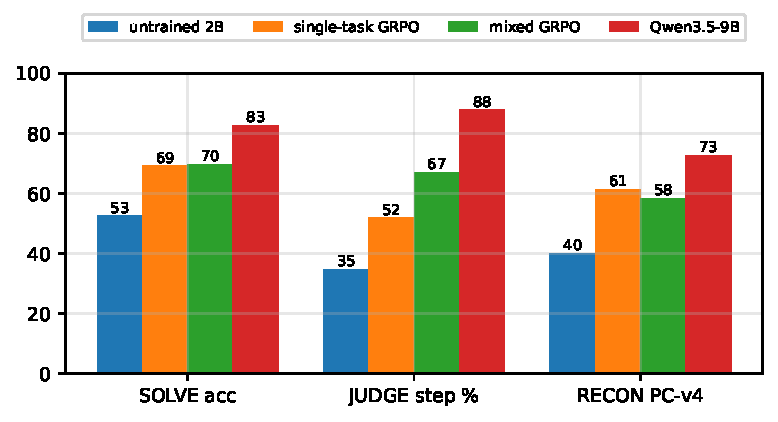
\includegraphics[width=0.7\linewidth]{figures/own_task_vs_9b.pdf}
\caption{Own-task scores: untrained 2B, single-task GRPO, mixed GRPO, and the untrained 9B.}
\end{figure}

\paragraph{How much of the gap to the 9B is closed.} Gap closed $=(\text{model}-\text{2B})/(\text{9B}-\text{2B})$:

\begin{center}\small
\begin{tabular}{lrr}
\toprule
Metric & Single-task specialist & Mixed model\\
\midrule
SOLVE accuracy & 55\% & 57\%\\
JUDGE error-finding & 32\% & 61\%\\
RECONSTRUCT PC-v4 & 66\% & 56\%\\
\bottomrule
\end{tabular}
\end{center}

\noindent On JUDGE the mixed model nearly matches the 9B: verdict accuracy 87.0 vs 87.6, and fewer false alarms
(7.5 vs 17.8).

\subsection{JUDGE by answer-key label}
\begin{table}[H]
\centering\small
\caption{JUDGE verdict accuracy by key label, and error-finding (200 questions each).}
\begin{tabular}{lrrr}
\toprule
Model & correct solutions: verdict & incorrect solutions: verdict & incorrect: verdict + step\\
\midrule
Untrained 2B & 62.7 & 65.9 & 34.8\\
SOLVE only & 76.5 & 67.5 & 43.5\\
JUDGE only & 87.0 & 70.0 & 52.0\\
RECONSTRUCT only & 52.5 & 84.0 & 49.0\\
Mixed & \textbf{92.5} & 81.5 & \textbf{67.0}\\
\bottomrule
\end{tabular}
\end{table}

\paragraph{Reading the table.}
\begin{itemize}
\item The RECONSTRUCT model's gain on incorrect solutions comes from answering ``incorrect'' more often; its accuracy
      on correct solutions falls to 52.5.
\item The mixed model improves on both kinds of solution.
\end{itemize}

\subsection{Sub-dimensions (27B judge, 0--4, gated answers count as 0)}
\begin{table}[H]
\centering\small
\begin{tabular}{lrrrrrrrr}
\toprule
Model & JUDGE V & L & E & M & RECON P & T & E & M\\
\midrule
Untrained 2B & 2.57 & 1.95 & 2.08 & 1.99 & 1.71 & 1.97 & 1.90 & 0.84\\
SOLVE only & 2.88 & 2.40 & 2.52 & 2.26 & 1.88 & 2.10 & 2.06 & 0.98\\
JUDGE only & 3.14 & 2.78 & 2.80 & 2.83 & 1.88 & 2.17 & 2.28 & 1.04\\
RECONSTRUCT only & 2.73 & 2.03 & 2.09 & 2.06 & \textbf{2.49} & \textbf{3.00} & \textbf{3.58} & 0.75\\
Mixed & \textbf{3.48} & \textbf{3.19} & \textbf{3.25} & \textbf{3.00} & 2.37 & 2.72 & 2.88 & \textbf{1.37}\\
\textit{Qwen3.5-9B} & 3.61 & 3.50 & 3.54 & 3.50 & 2.85 & 3.17 & 3.44 & 2.33\\
\bottomrule
\end{tabular}
\end{table}
\noindent
\begin{itemize}
\item The RECONSTRUCT specialist gains on fidelity and evidence use (P, T, E), but its mathematical validity drops
      (0.84 $\rightarrow$ 0.75).
\item The mixed model has the best validity of the 2B models (1.37).
\end{itemize}

\subsection{Behaviour: gates and answer length (test, all samples)}
\begin{table}[H]
\centering\small
\begin{tabular}{lrrrrrr}
\toprule
Model & \multicolumn{2}{c}{SOLVE} & \multicolumn{2}{c}{JUDGE} & \multicolumn{2}{c}{RECONSTRUCT}\\
\cmidrule(lr){2-3}\cmidrule(lr){4-5}\cmidrule(lr){6-7}
 & gate\,\% & mean tokens & gate\,\% & mean tokens & gate\,\% & mean tokens\\
\midrule
Untrained 2B & 6.8 & 8,089 & 13.8 & 5,087 & 12.6 & 5,337\\
SOLVE only & 1.4 & 8,643 & 11.8 & 5,613 & 11.5 & 5,734\\
JUDGE only & 4.0 & 5,518 & 1.2 & 3,017 & 16.0 & 5,287\\
RECONSTRUCT only & 1.1 & 5,291 & 3.8 & 5,026 & 3.8 & 2,236\\
Mixed & 1.0 & 9,114 & 1.8 & 6,751 & 5.5 & 7,793\\
\textit{Qwen3.5-9B} & 3.2 & 4,088 & 5.4 & 3,737 & 3.8 & 3,889\\
\bottomrule
\end{tabular}
\end{table}
\noindent
\begin{itemize}
\item JUDGE and RECONSTRUCT training shorten answers on their own tasks ($-41\%$ and $-58\%$).
\item The mixed model writes longer answers on every task (SOLVE $+13\%$, JUDGE $+33\%$, RECONSTRUCT $+46\%$).
\item No trained model has more than 0.5\% of answers capped at 32k.
\end{itemize}

\subsection{SOLVE answer types}
\begin{table}[H]
\centering\small
\begin{tabular}{lrrrrrr}
\toprule
Model & correct & wrong & unverified & gated & no answer & capped\\
\midrule
Untrained 2B & 52.6 & 20.8 & 16.2 & 6.8 & 3.6 & 0.1\\
SOLVE only (66) & 69.2 & 15.6 & 12.6 & 1.4 & 1.3 & 0.0\\
Mixed (75) & 69.8 & 16.4 & 11.4 & 1.0 & 1.0 & 0.4\\
\bottomrule
\end{tabular}
\end{table}
\noindent About 8 points of the SOLVE gain come from format fixes (gated or missing answers); about 9 come from
fewer wrong or undecidable answers.

%=====================================================================================================================
\section{Training dynamics}

\begin{figure}[H]
\centering
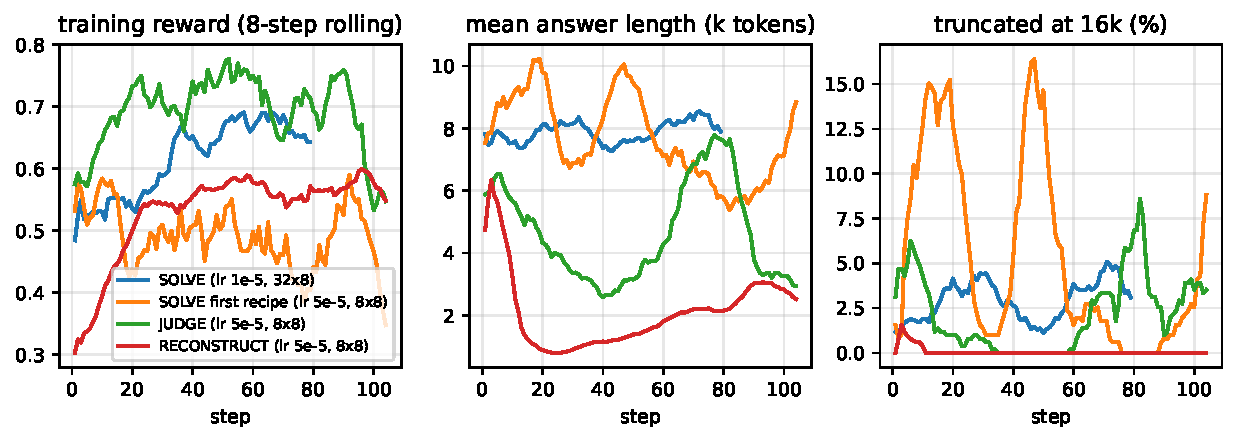
\includegraphics[width=\linewidth]{figures/curves_single.pdf}
\caption{Single-task runs. Rewards differ by task and are comparable only within a curve.}
\end{figure}

\begin{figure}[H]
\centering
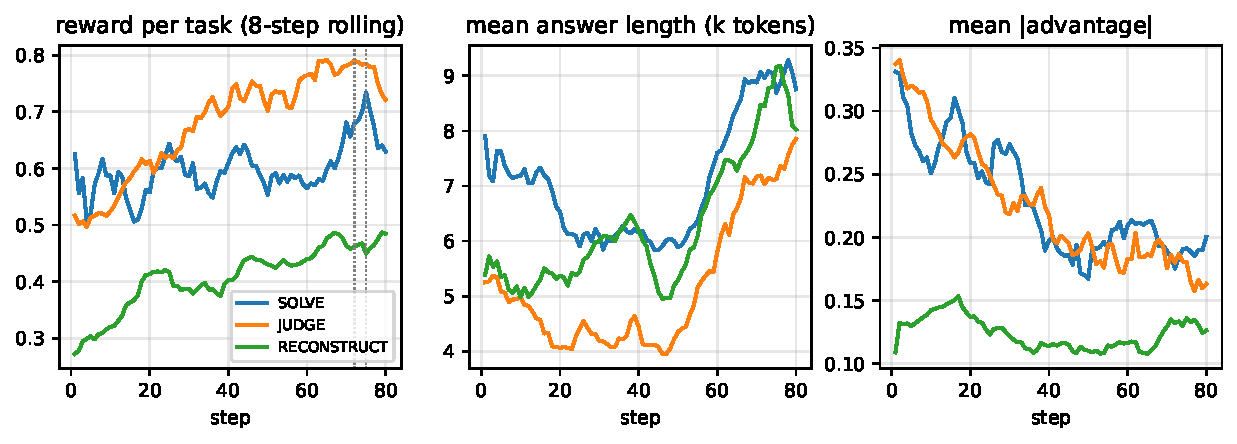
\includegraphics[width=\linewidth]{figures/curves_mixed.pdf}
\caption{Mixed run, per task. Dotted lines: steps 72 and 75.}
\end{figure}

\begin{table}[H]
\centering\small
\caption{Mixed run in 8-step blocks.}
\begin{tabular}{lrrrlr}
\toprule
Steps & SOLVE reward & JUDGE reward & RECON reward & length S / J / R & truncation\\
\midrule
1--8 & 0.62 & 0.52 & 0.31 & 7.1k / 4.9k / 5.1k & 1--5\%\\
17--24 & 0.62 & 0.62 & 0.42 & 6.1k / 4.3k / 5.4k & 0--1\%\\
41--48 & 0.59 & 0.75 & 0.44 & 6.0k / 4.1k / 5.0k & 0\%\\
65--72 & 0.68 & 0.79 & 0.46 & 9.0k / 7.0k / 8.4k & $\approx$4\%\\
73--80 & 0.63 & 0.72 & 0.49 & 8.8k / 7.9k / 8.0k & 4--7\%\\
\bottomrule
\end{tabular}
\end{table}

\noindent\textbf{Combined rolling reward} at the 8-step checks:

\begin{center}\small
\begin{tabular}{lrrrrrrrrr}
\toprule
Step & 16 & 24 & 32 & 40 & 48 & 56 & 64 & 72 & 80\\
\midrule
Combined gain & $+0.007$ & $+0.072$ & $+0.065$ & $+0.091$ & $+0.109$ & $+0.092$ & $+0.128$ & $+0.161$ & $+0.130$\\
\bottomrule
\end{tabular}
\end{center}

\noindent Its per-step maximum is $+0.174$, at step 75.

\paragraph{Observations.}
\begin{itemize}
\item \textbf{Reward scale:} RECONSTRUCT's mean $|\hat A|$ was about $2\times$ smaller than SOLVE's and JUDGE's
      (0.11--0.15 vs 0.20--0.34). That is below the planned $3\times$ threshold, so no per-task rescaling was
      applied.
\item \textbf{Length drift:} answer lengths rose for every task from step $\approx$57 at lr $2\times10^{-5}$. This is
      the same drift the lr $5\times10^{-5}$ runs showed.
\item \textbf{JUDGE early peak:} in its single-task run, JUDGE peaked early (dev best at step 26) and declined. The
      SOLVE and RECONSTRUCT rewards plateaued after steps $\approx$50 and $\approx$40.
\end{itemize}

%=====================================================================================================================
\section{The SOLVE story: why the first recipe failed and what fixed it}
\label{sec:solve}

\paragraph{First recipe} (lr $5\times10^{-5}$, 8$\times$8, 104 steps): test $-2.2$\ci{$-5.8$}{$+1.1$}. Diagnosis from
its 6,656 training rollouts:
\begin{itemize}
\item \textbf{Too little signal per step.} Questions whose answers differed fell from 5.5 to 3.8 of 8, so each update
      came from about 3 questions at a high lr.
\item \textbf{More wrong answers.} Wrong answers rose from 23\% to 33\% of rollouts. Truncation fell, but the formerly
      truncated answers now finished wrong. The rolling reward fell from 0.55 to 0.35.
\item \textbf{Little data.} Only 832 of 3,400 questions were seen.
\end{itemize}

\paragraph{Fixes and evidence.}
\begin{enumerate}
\item \textbf{Checker v3} (Section~\ref{sec:scoring}).
\item \textbf{32 questions $\times$ 8 answers per step}, so 18--25 questions per step carry a signal.
\item \textbf{lr probe}, at 32$\times$8, step 8, dev 200$\times$4:
  \begin{itemize}
  \item $10^{-5}$: $+3.8$\ci{$-0.2$}{$+7.6$};
  \item $2\times10^{-5}$: $+3.9$\ci{$+0.2$}{$+7.5$};
  \item the first recipe at step 26 was $-4.5$.
  \end{itemize}
  We chose $10^{-5}$, the literature value for LoRA ($\approx10\times$ the $10^{-6}$ used for full fine-tuning in
  DeepMath and DeepScaleR).
\item \textbf{Overlapped rollouts} (15 $\rightarrow$ 8 min/step); the log-prob gap stayed at 0.010--0.011.
\item \textbf{Result:} the rolling reward rose from 0.53 to 0.69 (step 66). Dev at step 66 was $72.4$ vs $52.4$
      ($+20.0$\ci{$+15.9$}{$+24.1$}); test $+16.6$.
\end{enumerate}

\paragraph{Deliberately not used:}
\begin{itemize}
\item difficulty filtering (user decision);
\item length penalties;
\item a longer cap: 16k already covers 99.3\% of the untrained model's correct answers.
\end{itemize}

\paragraph{Dev checkpoint scores of the other runs.}
\begin{itemize}
\item \textbf{JUDGE}, verdict + step (sum of two accuracies) at steps 26/52/78/104: \textbf{1.441}, 1.215, 1.302,
      1.034.
\item \textbf{RECONSTRUCT}, Jev score: 56.6, 62.2, 60.7, \textbf{63.1}.
\item \textbf{First SOLVE recipe}, checker v3: 47.9, 51.2, 49.4, \textbf{54.2} (untrained 52.4).
\end{itemize}

%=====================================================================================================================
\section{Comparison with published recipes}
\begin{table}[H]
\centering\small
\resizebox{\linewidth}{!}{%
\begin{tabular}{lllll}
\toprule
Recipe & lr & questions $\times$ answers / step & reward & notes\\
\midrule
Ours, SOLVE (new) & $10^{-5}$ LoRA & 32 $\times$ 8 & 1/0 verified & Dr.~GRPO, no KL, overlapped\\
Ours, mixed & $2\times10^{-5}$ LoRA & 30 $\times$ 8 (10/10/10) & per task & as above\\
DeepMath-1.5B (official code) & $10^{-6}$ full & 128 $\times$ 16, refills groups & $\pm1$ (math\_equal $\vee$ math-verify) & KL 0.001, $T$ 0.6, 24k\\
DeepScaleR-1.5B & $10^{-6}$ full & 128 $\times$ 8 & 1/0 & 8k$\rightarrow$16k$\rightarrow$24k\\
Dr.~GRPO paper & full & -- & 1/0 & no $\div$std, constant normalizer\\
TRL ``LoRA without regret'' & $\approx10^{-5}$ LoRA & 32--512 & -- & LoRA $\approx10\times$ full-FT lr\\
\bottomrule
\end{tabular}}
\end{table}

%=====================================================================================================================
\section{Limitations}
\begin{enumerate}
\item \textbf{One seed per model.} The confidence intervals cover question sampling only.
\item \textbf{The models use different recipes:}
  \begin{itemize}
  \item SOLVE: lr $10^{-5}$, 32$\times$8;
  \item mixed: lr $2\times10^{-5}$, 30$\times$8;
  \item JUDGE and RECONSTRUCT: lr $5\times10^{-5}$, 8$\times$8.
  \end{itemize}
  The cross-task and mixed-vs-specialist comparisons therefore mix task and recipe effects. In particular, the
  JUDGE specialist saw 208 JUDGE questions, against 750 for the mixed model.
\item \textbf{Different selection rules.} The mixed model's checkpoint was chosen by training reward without a dev
      check.
\item \textbf{One sample} per question for trained models on JUDGE and RECONSTRUCT.
\item \textbf{Judge dependence:} the judge-based metrics depend on the 27B judge's calibration ($r$ 0.94 / 0.84 vs
      DeepSeek).
\item \textbf{Unverifiable answers:} about 11--16\% of SOLVE answers stay unverified (forms that rules cannot check)
      and count as wrong for every model. Deltas are unaffected; absolute accuracy is underestimated.
\item \textbf{Longer answers:} the mixed model writes longer answers on every task.
\end{enumerate}

%=====================================================================================================================
\section{Compute}
\begin{itemize}
\item \textbf{Hardware:} the Turing cluster, NVIDIA L40S (46\,GB).
\item \textbf{GPU limits:} at most 6 GPUs at once, then at most 4 from 2026-10-07.
\item \textbf{Ledger:} 234 GPU-hours used of the 500 approved, covering all work (baselines, judge calibration, the
      first matrix, the SOLVE probes and run, the mixed run, all evaluations and judging). 266 remain.
\item \textbf{Jev API:} JUDGE and RECONSTRUCT rewards and RECONSTRUCT dev scoring, a few US dollars in total.
\end{itemize}

%=====================================================================================================================
\section{Reproducibility}
\begin{verbatim}
# SOLVE model (lr 1e-5, 32x8), end to end from the workstation
nohup bash scripts/solve_grpo_pipeline.sh \
    > artifacts/opd/evals/solve-pipeline.log 2>&1 &
# Mixed model (1/3 each, lr 2e-5, 30x8), end to end
NODE=node07 nohup bash scripts/mixed_grpo_pipeline.sh \
    > artifacts/opd/evals/mixed-pipeline.log 2>&1 &

# one run by hand (2 GPUs: vLLM + trainer)
python3 scripts/turing/launch.py submit --name <run> --gpus 2 --hours 14 --node <node> -- \
  python scripts/turing/opd_run.py --task {solve|judge|reconstruct|mixed} --config grpo \
    --steps <n> --set prompts_per_step=<32|30> --set optimizer.lr=<1e-5|2e-5> \
    --set optimizer.warmup_steps=5 --set async_rollouts=true \
    --set best_window=8 --set best_keep=3 --student-port <port> \
    --out /scratch/mukund.hebbar/anlp-opd/v3/<run>

# evaluation, 27B judging, calibration, reports
python scripts/turing/eval_matrix.py --name <n> --adapter <adapter> --split test \
    --samples 4 --samples-tasks solve --out <dir>
python scripts/turing/qwen_judge_run.py --eval-dir test:<dir>/s0 --out <log>/answers.jsonl
uv run python scripts/qwen_judge_calibration.py score <dir>/s0
uv run python scripts/rescore_solve.py <eval dirs>          # after any checker change
SOLVE_SEL=66 MIXED_SEL=75 uv run python scripts/report_grpo_matrix.py
uv run python scripts/make_report_figures.py
uv run python -m unittest discover -s tests                 # 229 tests
\end{verbatim}

\paragraph{Files.}
\begin{itemize}
\item \textbf{Test answers and scores:} \texttt{artifacts/baselines/final-v3/test/}, in the folders
  \begin{itemize}
  \item \texttt{v3-pass4-2b} (untrained 2B) and \texttt{v3-pass4-9b} (9B);
  \item \texttt{v3-grpo-lr1e-5-solve-step66} (SOLVE);
  \item \texttt{v3-drgrpo-judge-step26} (JUDGE) and \texttt{v3-drgrpo-reconstruct-step104} (RECONSTRUCT);
  \item \texttt{v3-grpo-mixed-lr2e-5-step75} (mixed);
  \item \texttt{v3-drgrpo-solve-step104} (first SOLVE recipe).
  \end{itemize}
\item \textbf{Training metrics and checkpoint records:} \texttt{artifacts/opd/evals/\{solve-p1-lr1e-5, mixed-lr2e-5,
      v3-drgrpo-dev\}}.
\item \textbf{Adapters} (Turing scratch):
  \begin{itemize}
  \item SOLVE: node11 \texttt{v3/solve-p1-lr1e-5/adapters/best-step66}, also copied to
        \texttt{\textasciitilde/anlp-project/runs-out};
  \item mixed: node07 \texttt{v3/mixed-lr2e-5/adapters/best-step75};
  \item JUDGE: node11 \texttt{v3/v3-drgrpo-judge-r2/adapters/step26};
  \item RECONSTRUCT: node07 \texttt{v3/v3-drgrpo-reconstruct/adapters/step104}.
  \end{itemize}
\item \textbf{Code:}
  \begin{itemize}
  \item \texttt{src/anlp\_project/}: \texttt{opd\_train.py} (GRPO loop, overlap, per-task metrics, best checkpoints),
        \texttt{opd.py} (configs, mixed prompts), \texttt{rewards.py}, \texttt{solution\_verification.py} (checker
        v3), \texttt{strict\_gates.py}, \texttt{jev\_judging.py}, \texttt{qwen\_judging.py};
  \item scripts in \texttt{scripts/} and \texttt{scripts/turing/}.
  \end{itemize}
\end{itemize}

\appendix
\section{Exact run configurations (\texttt{config.json} of each run)}
Each file is as written by the trainer at the start of its final chunk (one key per line); \texttt{overrides}
lists the command-line \texttt{--set} values. The fields \texttt{teacher}, \texttt{objective},
\texttt{loss\_normalization}, \texttt{topk\_*}, \texttt{sft\_mix}, \texttt{verdict\_reward} and
\texttt{teacher\_*} are inherited from the on-policy-distillation configuration and are \emph{unused} when
\texttt{method} is \texttt{grpo}. The GRPO loss is the one in Section~4, with \texttt{norm\_tokens} as the
constant normalizer.

\subsection{SOLVE (new recipe), chunk resumed at step 9}
{\scriptsize\verbatiminput{configs/solve_new.txt}}
\subsection{Mixed run}
{\scriptsize\verbatiminput{configs/mixed.txt}}
\subsection{JUDGE}
{\scriptsize\verbatiminput{configs/judge.txt}}
\subsection{RECONSTRUCT}
{\scriptsize\verbatiminput{configs/reconstruct.txt}}
\subsection{SOLVE (first recipe)}
{\scriptsize\verbatiminput{configs/solve_old.txt}}

\section{References}
\begin{itemize}
\item Liu et al., \emph{Understanding R1-Zero-Like Training: A Critical Perspective} (Dr.~GRPO), arXiv 2503.20783.
\item He et al., \emph{DeepMath-103K}, arXiv 2504.11456; official code \url{https://github.com/zwhe99/DeepMath}.
\item Luo et al., \emph{DeepScaleR: Surpassing O1-Preview with a 1.5B Model by Scaling RL} (2025).
\item Cheng et al., \emph{Revisiting RL for LLM Reasoning from a Cross-Domain Perspective} (GURU), arXiv 2506.14965.
\item Li et al., \emph{Can One Domain Help Others? A Data-Centric Study on Multi-Domain Reasoning via RL}, arXiv
      2507.17512.
\item \emph{Advancing General-Purpose Reasoning Models with Modular Gradient Surgery}, arXiv 2602.02301.
\item \emph{SFT Conflicts, RL Coexists: Multi-Task Learning for LLMs}, arXiv 2608.03573.
\item Hugging Face TRL, \emph{LoRA Without Regret}; \texttt{math-verify}; OpenMathInstruct grader (via DeepMath).
\end{itemize}

\end{document}
